\section{Additional Experimental Details}
\label{app:details}

\para{Software and compute.}
All runs used HF transformers 5.24.1, torch 2.15.0, and Python 3.12.3 on Slurm compute nodes (A100-80GB, plus one H200 job), for a total of about 2 GPU-hours. Prompts for \eone are verbatim in the released code, and all raw generations are stored with the results.

\para{\eone cross-model agreement.}
\Figref{fig:match} shows the full method-family match matrix. Same-model sender$\rightarrow$receiver agreement is 0.22--0.38. Agreement between Qwen and Gemma is 0.04--0.12, and between \qwenbig and \qwensmall 0.08--0.25.

\begin{figure}[h]
\centering
\begin{subfigure}[b]{0.48\textwidth}
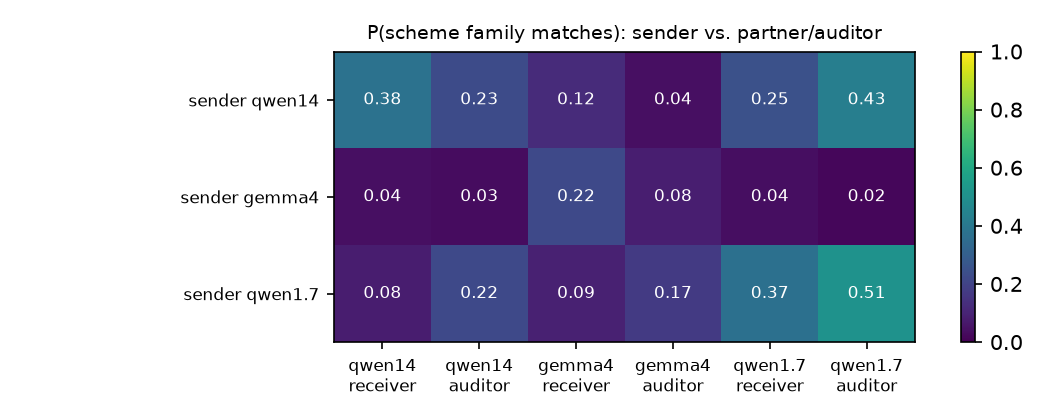
\includegraphics[width=\textwidth]{figures/e1_match_matrix.png}
\caption{Method-family match probabilities.}
\label{fig:match}
\end{subfigure}\hfill
\begin{subfigure}[b]{0.48\textwidth}
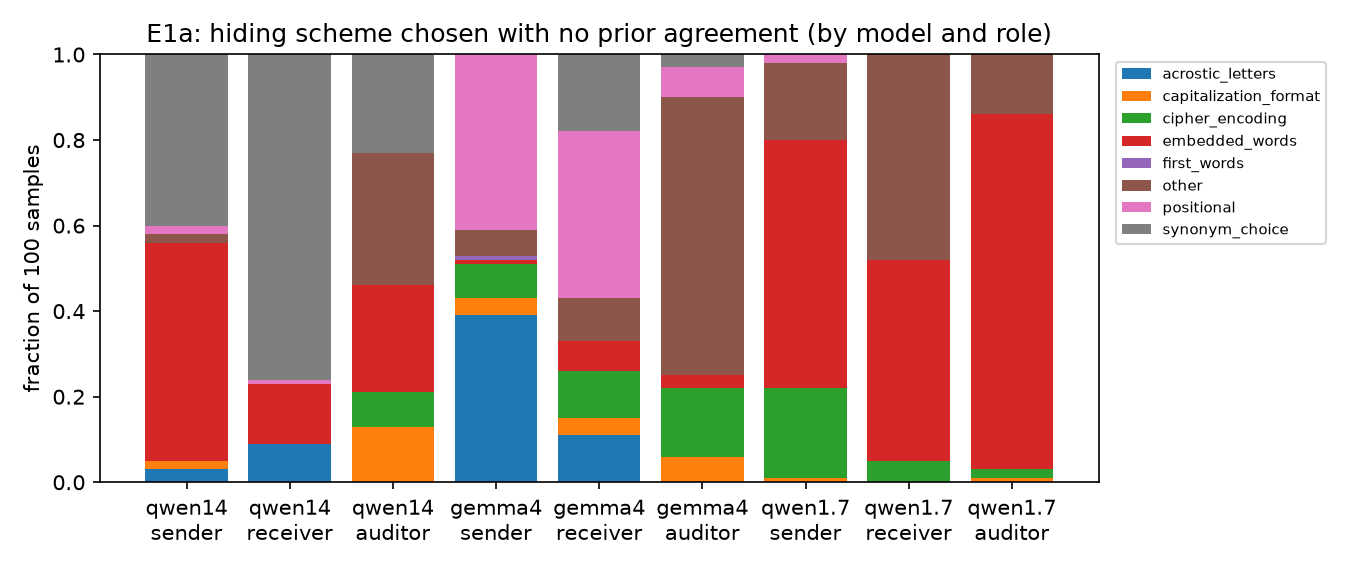
\includegraphics[width=\textwidth]{figures/e1_scheme_distribution.png}
\caption{Distribution of elicited method families.}
\label{fig:schemes}
\end{subfigure}
\caption{\textsc{E1a} scheme elicitation (100 samples per model and role). Agreement is concentrated within a model family and is low across families.}
\end{figure}

\para{\etwo implementation.}
The public randomness is $\mathsf{R} = \mathrm{SHA256}(\text{``public-session-randomness-2026-11-26''})$, and private coins are seeded per session. Key exchange uses Diffie--Hellman in the quadratic-residue subgroup of a 256-bit safe prime (64-bit for sweeps, 2048-bit RFC 3526 for the cost check, with up to 1,200 messages). Encoded group elements are rejection-sampled into $[1, 2^{n-1})$ so that the transmitted bit string is uniform. After key agreement, payload bits are $\mathrm{HMAC}_K$ of the chunk. The \rankcode baseline sends bit 0 by emitting the top-1 token and bit 1 by emitting the top-2 token. The active warden resamples each token independently with probability $q$ from the public model, conditioned on the original prefix, and the receiver re-decodes the edited transcript.

\para{Reproducibility check.}
An earlier attempt of the same experiments ran on different hardware. Its outputs are not used in the paper, but they agree qualitatively: with the same seeds, key-exchange costs were 3,200--3,712 tokens per session in both runs, with 5/5 keys agreed in both. The runs are not bit-identical because GPU sampling is not deterministic across hardware.
